% !TEX root = ../main.tex
\section{Results and Conclusions}
\label{14::results_and_conclusions}
    The FMT efficiency is discussed in the first section, including a brief study of it.
    Then, the second section delves into the acceptance correction results, based on the methodology described in Section \ref{13.40::acceptance_correction}.
    Following that, the study results are discussed in detail, and the conclusions of the study follow shortly thereafter.

    % Run configuration.
    All Figures in this section that show results for data are from RG-F run 12016.
    For this run, a gas H2 target was used.
    The beam energy was set to $10.4$ GeV, and the luminosity to $250$ nA.
    The solenoid field was set to an inbending polarity ($-0.75$), and the torus to its regular polarity of $-1$.
    The run has a total of $10,046,225$ events.

    % !TEX root = ../main.tex
\subsection{FMT Efficiency}
\label{14.10::fmt_efficiency}
    % Low FMT efficiency + list sources.
    Compared to the alignment work described in Section \ref{12::fmt_alignment_and_reconstruction}, a low FMT is observed in this analysis.
    This is evident in Figure \ref{fig::14.10::vz_012933}.
    Upon inspection, three causes can be attributed to this: the application of incorrect alignment constants, a geometry effect, and a general FMT offline reconstruction issue.

    \begin{figure}[b!]
        \centering\frame{
        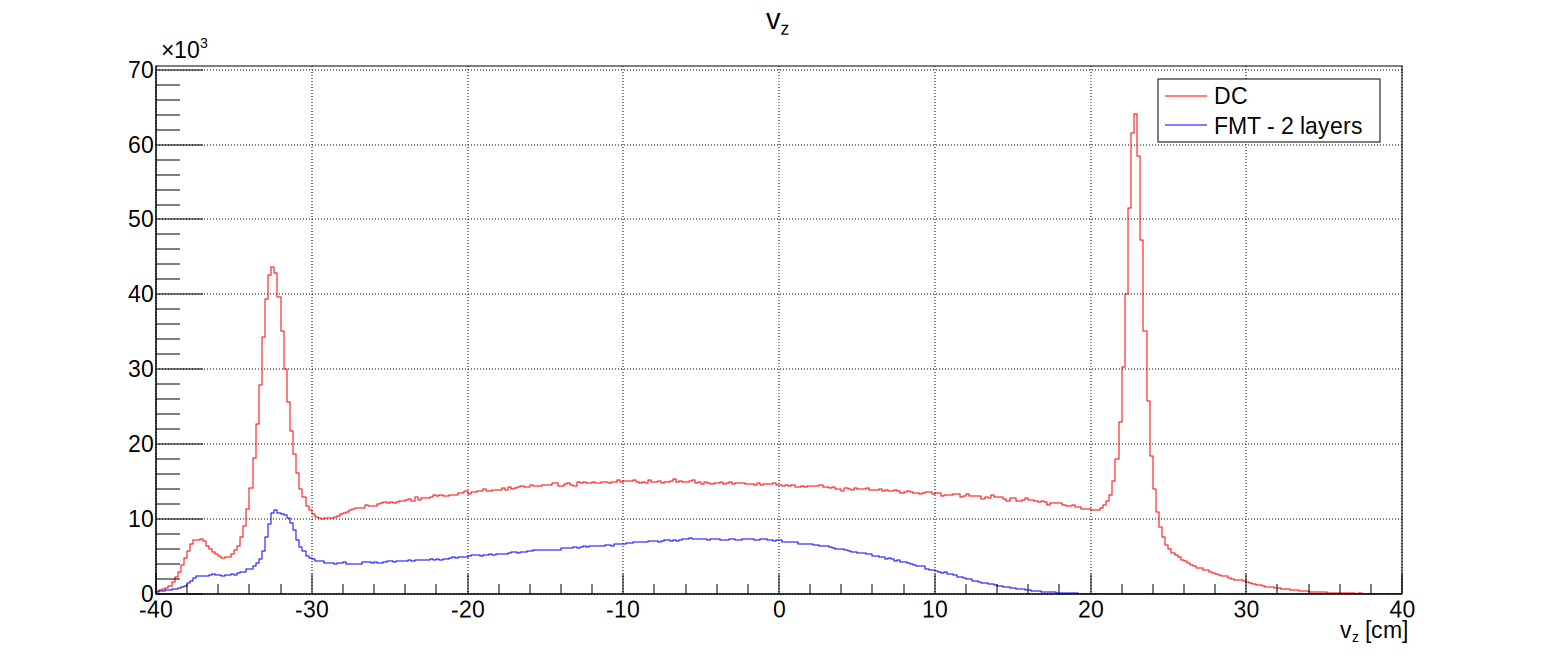
\includegraphics[width=\textwidth]{10vz_012933.pdf}}
        \caption[$v_z$ for DC and FMT, run 12933]{$v_z$ for DC (in red) and FMT (in blue). Summer 2020 data, run 12933. The wide peaks in FMT suggest an uncorrected misalignment.}
        \label{fig::14.10::vz_012933}
    \end{figure}

    In this section, we extensively discussed the efficiency of the FMT detector, addressing alignment issues, as well as the impact of implementing a geometry cut.
    The key findings can be summarized as follows: despite applying corrections, the FMT efficiency for 3-layer tracks remained low, rendering them impractical for exclusive use.
    However, by switching to Spring 2020 data and applying the geometry cut, significant improvements were observed in the detection of trigger electrons and pions.
    Moreover, we thoroughly examined the correlation between efficiency and various variables, namely $v_z$, $\theta$, $\phi$, and $p$.
    The results were as anticipated: strong correlations were observed for $v_z$ and $\theta$, while no significant correlation was found for $\phi$ or $p$.
    These findings provide valuable insights into the performance and limitations of FMT, paving the way for an acceptance correction study and the following work.

    % !TEX root = ../main.tex
\subsubsection{Alignment Effect}
\label{14.11::alignment_effect}
    % Introduction: The problem.
    The data from the RG-F experiment is divided based on the season in which the runs take place, namely Spring 2020 and Summer 2020.
    According to the run group's guidelines, it is recommended to use Summer data as it has undergone more calibration compared to the Spring data.
    However, the calibration work conducted so far does not include the FMT detector, resulting in a significant misalignment effect.

    % Cause of the problem.
    Through simple visual inspection, two distinct peaks can be clearly observed between $z = -36$ cm and $z = -30$ cm in Figure \ref{fig::12.41::dc_vs_fmt_vz_11983}.
    The leftmost peak corresponds to the scattering chamber window, while the second peak corresponds to the RG-F target window.
    These peaks appear merged in Figure \ref{fig::14.10::vz_012933}.
    As discussed in Section \ref{12::fmt_alignment_and_reconstruction}, this issue arises due to the lack of correction for FMT misalignments.

    % Solution.
    The simplest solution is to utilise Spring data.
    Although more calibration work has been performed on the Summer data, it mainly pertains to the CD, which is not used in this analysis.
    Figure \ref{fig::14.11::vz_012016} depicts the same $v_z$ plot from Spring 2020 run 12016, where both peaks are clearly visible.
    This indicates that the misalignment issue has been appropriately addressed in that particular run.

    \begin{figure}[t!]
        \centering\frame{
        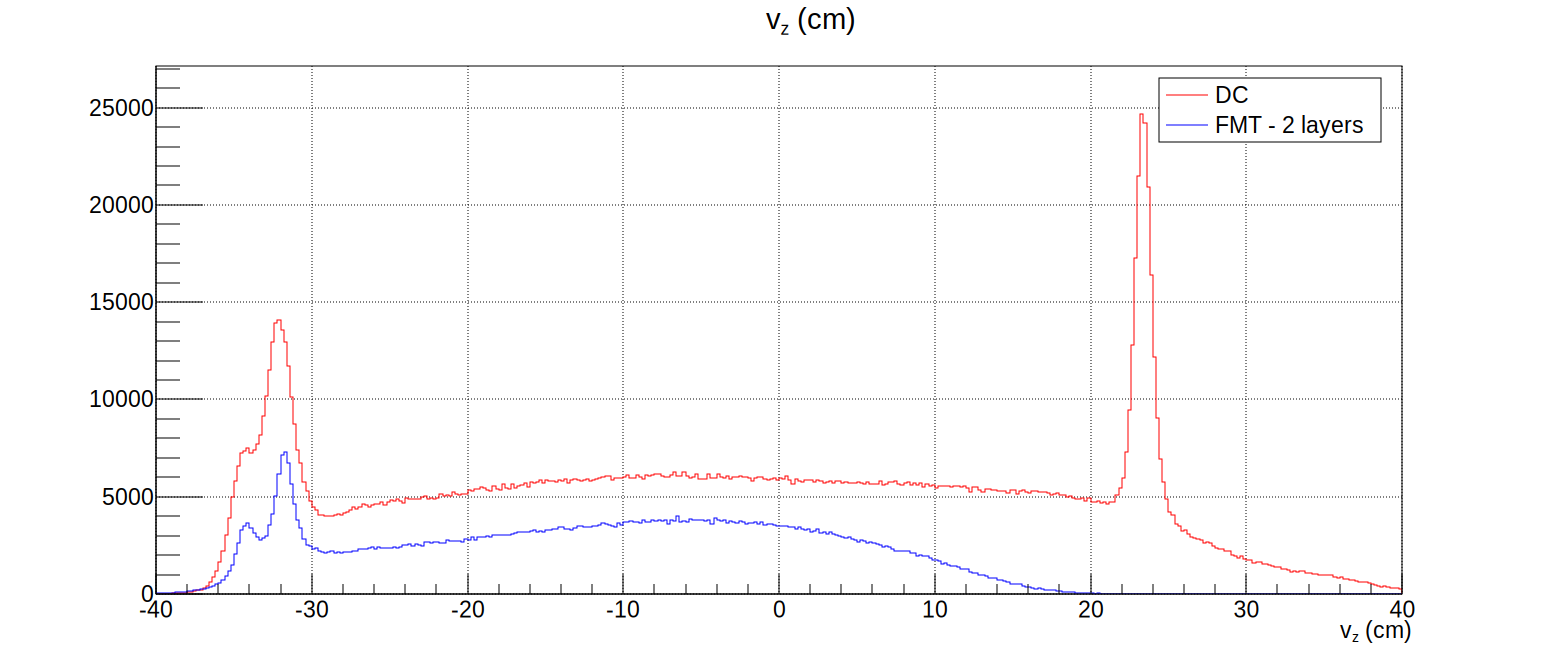
\includegraphics[width=\textwidth]{11vz_012016.pdf}}
        \caption[$v_z$ for DC and FMT, run 12016]{$v_z$ for DC (in red) and FMT (in blue).
        Spring 2020 data, run 12016. The upstream twin peaks can be clearly distinguished, suggesting a correct misalignment correction.
        Source: Own elaboration, using the \href{https://github.com/bleaktwig/clas12-rge-analysis}{clas12-rge-analysis} software.}
        \label{fig::14.11::vz_012016}
    \end{figure}

    % !TEX root = ../main.tex
\subsubsection{Geometry Effect}
\label{14.12::geometry_effect}
    % The effect has already been presented and discussed before, so we're brief.
    This problem has already been extensively discussed in section \ref{12.42::geometry_effect}.
    In summary, the FMT detector is located at approximately $z \approx 26$ cm, and it exhibits poor performance for targets located too close to it.
    The strength of this effect can be quantified by applying the geometry cut described by Equation \eqref{eq::12.42::fmt_geometry_cut} to both the DC and FMT tracks.
    Figure \ref{fig::14.12::vz_012016_geomcut} illustrates the impact of this cut on both the DC and FMT tracks when applied to figure \ref{fig::14.11::vz_012016}.
    The effect of the cut on a $v_z$ vs $\theta$ plot can be observed in Figure \ref{eq::12.42::vz_vs_theta}.

    Based on this cut and the FMT's position along the $z$-axis, subsequent plots will be confined to the range $-30 \text{cm} < v_z < 20 \text{cm}$.

    \begin{figure}[h!]
        \centering\frame{
        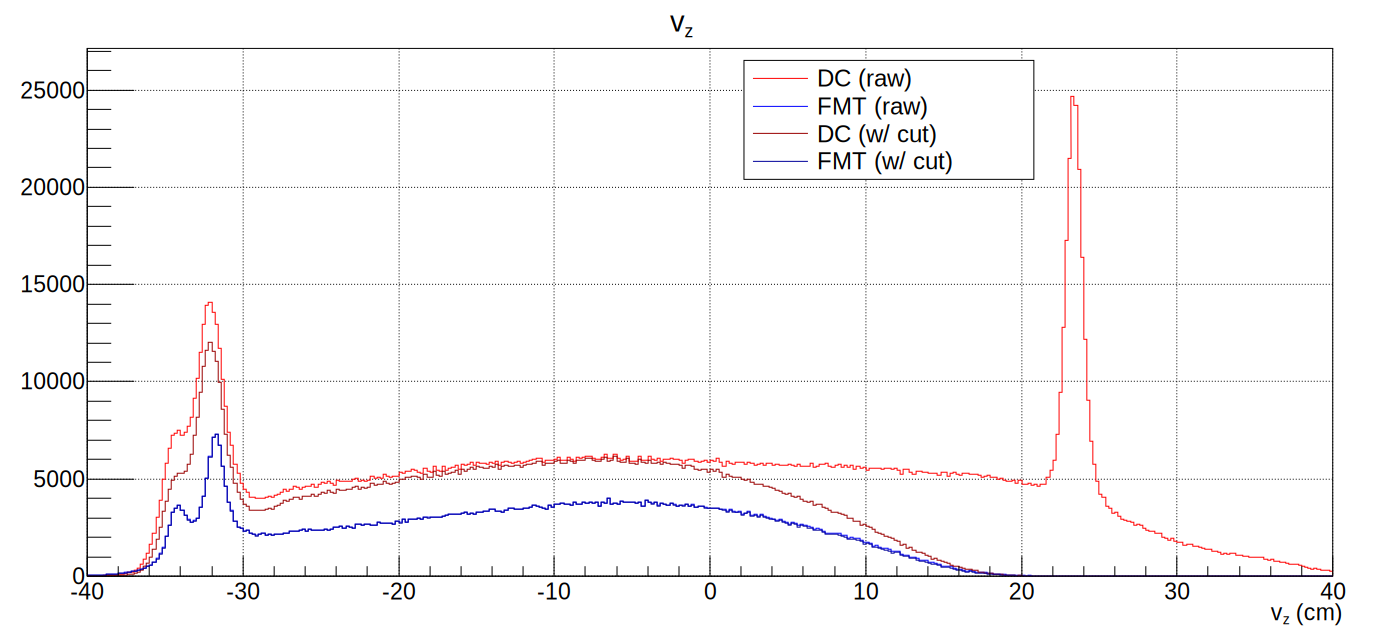
\includegraphics[width=\textwidth]{12vz_012016_geomcut.pdf}}
        \caption[$v_z$ for DC and FMT, w/ and w/out the geometry cut, run 12016]{$v_z$ for DC without the geometry cut (in red), with it (in dark red), for FMT without it (in blue), and with it (in dark blue).
        Spring 2020 data, run 12016.
        The effect is very clear on DC tracks, yet it almost doesn't affect FMT tracks.
        Source: Own elaboration, using the \hyperlink{github.com/bleaktwig/clas12-rge-analysis}{clas12-rge-analysis} software.}
        \label{fig::14.12::vz_012016_geomcut}
    \end{figure}

    % !TEX root = ../main.tex
\subsubsection{Reconstruction Effect}
\label{14.13::reconstruction_effect}
    Even after correcting for both the alignment and geometry issues, the FMT still exhibits lower efficiency compared to what was observed during alignment (compare Figure \ref{fig::14.12::vz_012016_geomcut} with Figure \ref{fig::12.43::dc_vs_fmt_vz_11983_corrected}).
    After conducting a thorough study, it was determined that this effect is not correlated with the run number, beam energy, or beam luminosity.
    Consequently, it can be concluded that the issue is not caused by hardware problems or run conditions.

    Based on these findings, the logical conclusion is that the effect stems from a general issue in the FMT offline reconstruction for data.
    Identifying and rectifying this issue would require a larger project beyond the scope of this thesis and is therefore left as future work.
    For the purposes of this analysis, we will rely on a large number of events to minimize any statistical deficiencies.

    % !TEX root = ../main.tex
\subsubsection{Efficiency Study}
\label{sssec::efficiency_study}
% --+ Integrated. +---------------------------------------------------------
    With all these effects accounted for, we can proceed to study the efficiency in detail.
    First, if we define FMT efficiency as the percentage of DC tracks that get accepted by FMT, we get table \ref{tab::fmt_efficiency_study} for runs 12933 (Summer 2020) and 12016 (Spring 2020).

    \begin{center}
        \begin{tabularx}{0.70\textwidth}{Xr|rrcrr}
            & & \multicolumn{2}{l}{\textbf{Run 12933}}  & & \multicolumn{2}{l}{\textbf{Run 12016}} \\
                             &          & raw  & w/ cut   & & raw  & w/ cut   \\
            \hline
            \textbf{$e^-$}   & 2 layers & 25.1\% & 37.5\% & & 32.7\% & 53.7\% \\
                             & 3 layers &  5.6\% &  8.5\% & &  9.9\% & 16.4\% \\
            \hline
            \textbf{$\pi^+$} & 2 layers &  6.5\% & 13.7\% & & 11.1\% & 28.0\% \\
                             & 3 layers &  0.3\% &  0.7\% & &  1.0\% &  2.7\% \\
            \hline
            \textbf{$\pi^-$} & 2 layers &  5.6\% & 14.2\% & &  8.9\% & 29.5\% \\
                             & 3 layers &  0.3\% &  0.7\% & &  0.9\% &  2.9\%
        \end{tabularx}
        \label{tab::fmt_efficiency_study}
    \end{center}

    % TODO. Change percentages based on new table.
    By switching from Summer to Spring data, we see a $\sim32\%$ increase in trigger electrons detected, and a $\sim36\%$ in all particles.
    Then, by applying the geometry cut in $v_z$ and $\theta$, $\sim64\%$ more trigger electrons are detected (for a $\sim184\%$ total increase), and $\sim126\%$ more particles in general are detected (for a $\sim207\%$ total increase).

% --+ Separated. +----------------------------------------------------------
    We can then check how the efficiency changes as result of the corrections.
    Due to the geometric cut, we expect a strong dependency on $v_z$ and $\theta$, and at most a weak one on $\phi$ and $p$.
    This is what we see in data, as is shown in figure \ref{fig::fmt_efficiencies}.

    % TODO. Explain the loss of dips in $\phi$ efficiency.

    \begin{figure}[t!]
        \centering\frame{
        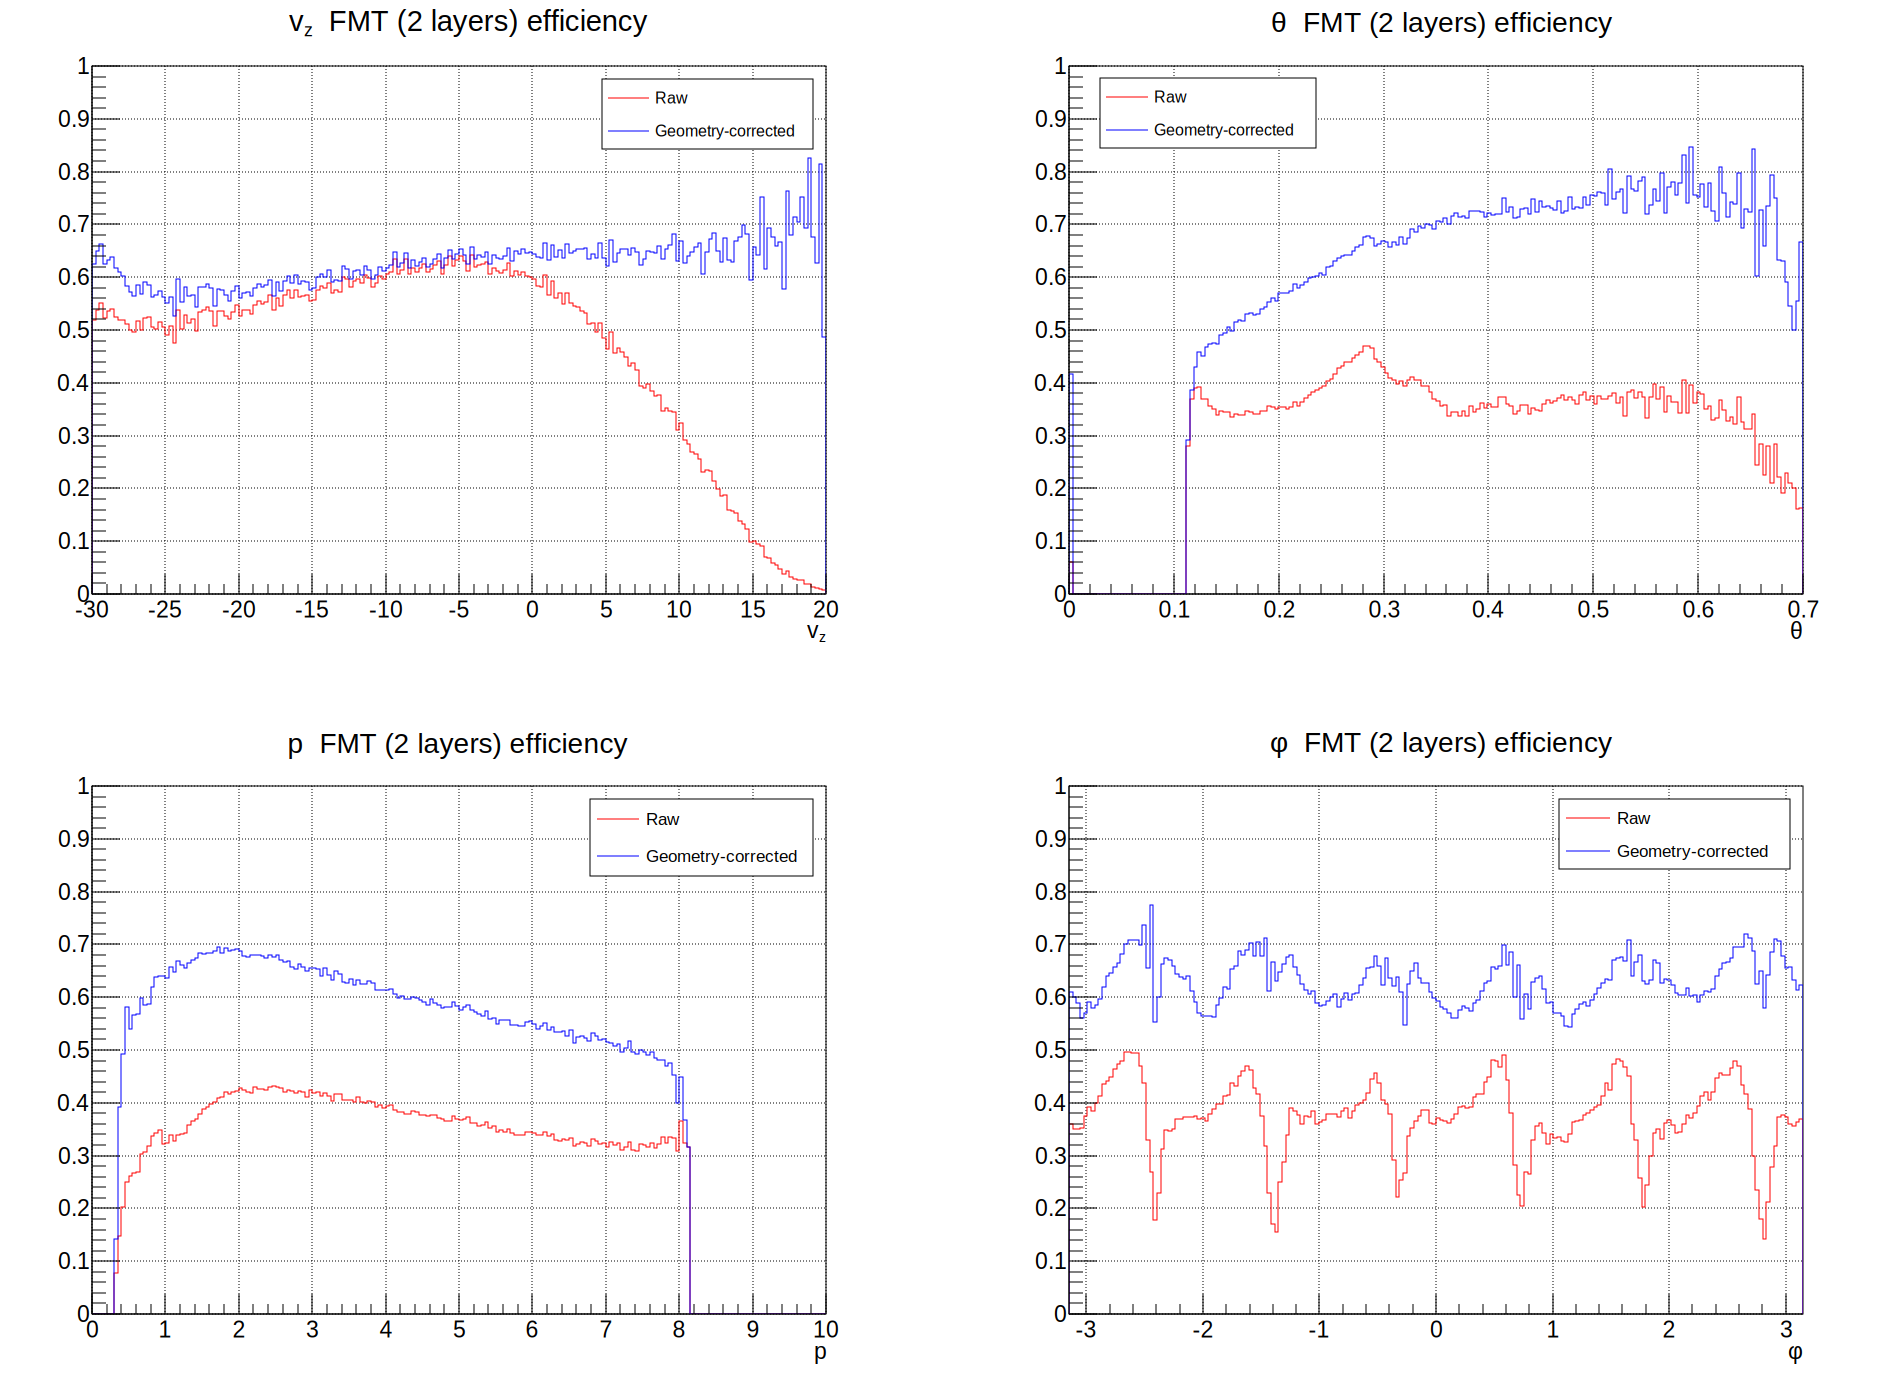
\includegraphics[width=\textwidth]{14efficiencies.pdf}}
        \caption[$v_z$, $\theta$, $\phi$, and $p$ efficiencies for FMT tracks, run 12016]{$v_z$, $\theta$, $\phi$, and $p$ efficiencies for FMT tracks. FMT Efficiency is defined as the percentage of DC tracks that are detected by 2 FMT layers. Run 12016.}
        \label{fig::fmt_efficiencies}
    \end{figure}


    % !TEX root = ../main.tex
\subsection{Acceptance Correction Results}
\label{14.20::acceptance_correction_results}
    DC and FMT acceptances were obtained by following the procedure described in Section \ref{13.13::acc_corr}.
    In this section, we will study the acceptance percentage for each electron and hadronic variable.
    These numbers represent the percentage of thrown particles that were detected by the DC and by 2 or 3 FMT layers in addition to DC in the GEMC simulation.

    Since they represent the acceptance percentage, all plots display a calculated division as follows
    \begin{equation}
        y_\text{acc} = \frac{y_r}{y_t},
        \label{eq::14.20::acc}
    \end{equation}
    where $y_\text{acc}$ is the percentage of accepted particles, $y_r$ is the number of reconstructed particles by the studied detector in the GEMC simulation, and $y_t$ is the number of particles thrown by LEPTO.

    Then, to propagate the error of $y_r$ ($e_d$) and $y_t$ ($e_t$) to $y_\text{acc}$ ($e_\text{acc}$), we have
    \begin{align}
        e_\text{acc} &= \delta \left(\frac{y_r}{y_t}\right)
        \nonumber \\
        &= y_\text{acc} \cdot \sqrt{
            \left( \frac{e_r}{y_r} \right)^2 + \left( \frac{e_t}{y_t} \right)^2
        },
        \nonumber
        \intertext{since $y_t$ is the number of trials, we can assume $e_t = 0$, and thus}
        &= y_\text{acc} \cdot \frac{e_r}{y_r}.
        \label{eq::14.20::acc_error_estimation}
    \end{align}

    From the Central Limit Theorem, assuming a normal distribution, the variance $e_r^2$ is given by
    \begin{equation*}
        e_r^2 = y_t \cdot y_\text{acc} (1 - y_\text{acc}).
    \end{equation*}

    Replacing this in Equation \eqref{eq::14.20::acc_error_estimation}, we obtain
    \begin{equation*}
        e_\text{acc} = y_\text{acc} \cdot \frac{\sqrt{y_t y_\text{acc}(1 - y_\text{acc})}}{y_r}.
    \end{equation*}

    Now, replacing $y_\text{acc}$ with its definition from Equation \eqref{eq::14.20::acc}, we arrive at the final error expression
    \begin{equation}
        e_\text{acc} = \sqrt{\frac{y_\text{acc}(1-y_\text{acc})}{y_t}}.
        \label{eq::14.20::acc_error}
    \end{equation}

    % !TEX root = ../main.tex
\subsubsection{Electron Variables}
\label{14.21::electron_variables}
    First, we'll study the $Q^2$ and $\nu$ acceptances for the scattered $e^-$.
    $Q^2$ and $\nu$ acceptances are presented in Figure \ref{fig::14.21::electron_acc}.
    Each one is presented in integrated kinematical region for the other variable.

    \textbf{TODO. Say something?}



    \begin{figure}
        \centering
        % Q2.
        \begin{subfigure}[b]{0.49\textwidth}
            \centering
            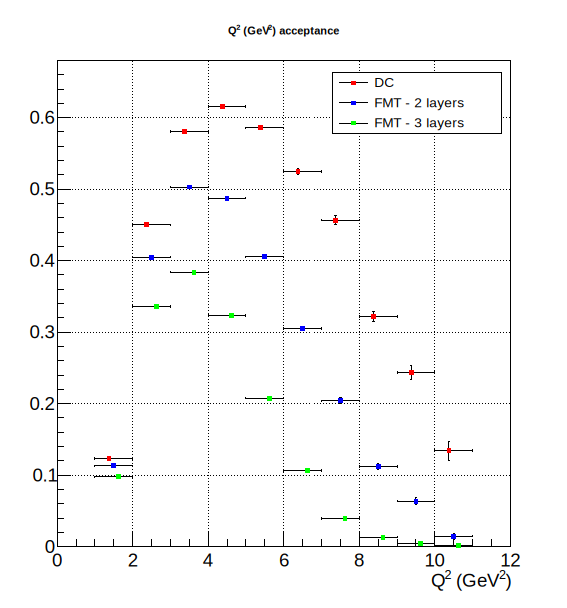
\includegraphics[width=\textwidth]{21q2_acc.pdf}
            \caption{$Q^2$ acceptance.}
            \label{fig::14.21::q2_acc}
        \end{subfigure}
        \hfill
        % nu.
        \begin{subfigure}[b]{0.49\textwidth}
            \centering
            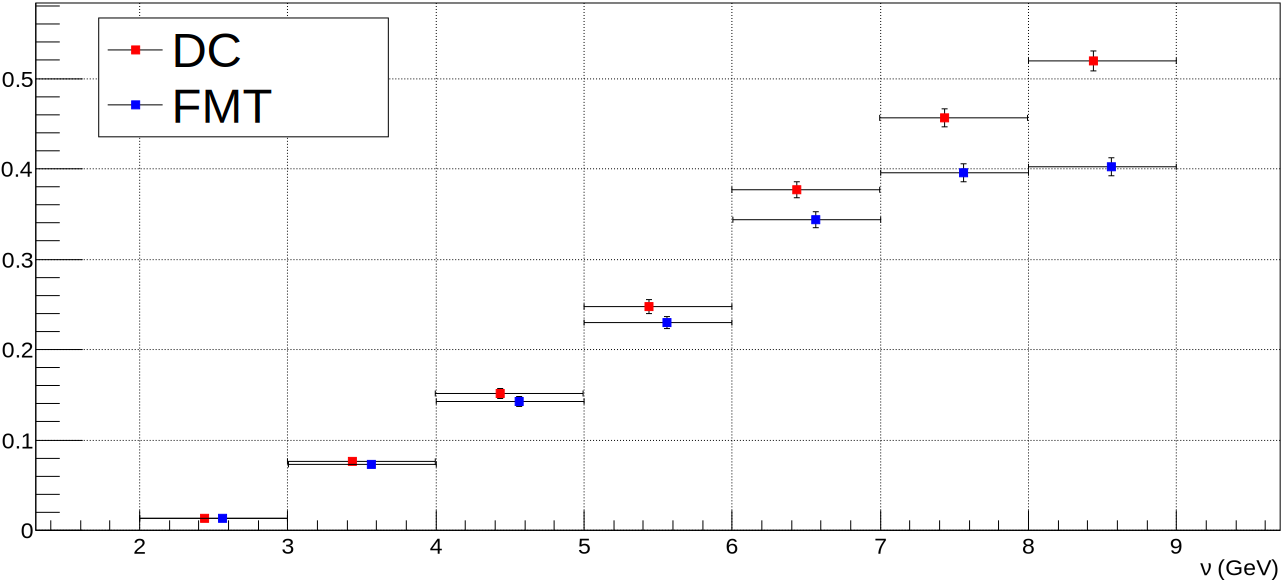
\includegraphics[width=\textwidth]{21nu_acc.pdf}
            \caption{$\nu$ acceptance.}
            \label{fig::14.21::nu_acc}
        \end{subfigure}
        \caption[Electron variables acceptance.]{Electron variables acceptance.
        $\nu$ is integrated in \ref{fig::14.21::q2_acc}, and $Q^2$ is integrated in \ref{fig::14.21::nu_acc}.
        The bin markers are slightly shifted in $x$ to improve legibility.
        Source: Own elaboration, using the \href{https://github.com/bleaktwig/clas12-rge-analysis}{clas12-rge-analysis} software.}
        \label{fig::14.21::electron_acc}
    \end{figure}

    % !TEX root = ../main.tex
\subsubsection{Hadronic Variables}
\label{14.22::hadronic_variables}
    The acceptance of the hadronic variables $z_h$, $p_T^2$, and $\phi_{PQ}$ for $e^-\pi^+$ and $e^-\pi^-$ are presented in Figure \ref{fig::14.22::hadronic_acc}.
    Each one is presented in integrated kinematical region for all electron variables and other hadronic variables.

    % Lower acceptance.
    It's worth noting that these acceptances are lower than those for electron variables.
    This is to be expected, since they require both the trigger electron and at least one hadron to be accepted by the detector.
    This same effect is seen in the $e^-\pi^+$ and $e^-\pi^-$ entries presented in the efficiency Table \ref{tab::14.14::fmt_efficiency_study}.

    % Particle charge-dependent acceptance.
    % TODO. Add phi vs theta (positive particles) plot and explain the difference in acceptances between pi+ and pi- based on that.

    \begin{figure}
        \centering
        % zh pi+.
        \begin{subfigure}[b]{0.49\textwidth}
            \centering
            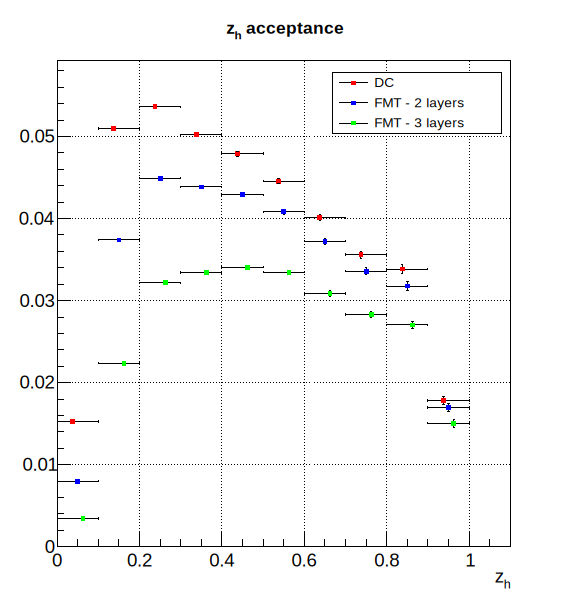
\includegraphics[width=\textwidth]{22zh_acc_211.pdf}
            \caption{$z_h$ acceptance for $e^-\pi^+$.}
            \label{fig::14.22::zh_acc_211}
        \end{subfigure}
        \hfill
        % zh pi-.
        \begin{subfigure}[b]{0.49\textwidth}
            \centering
            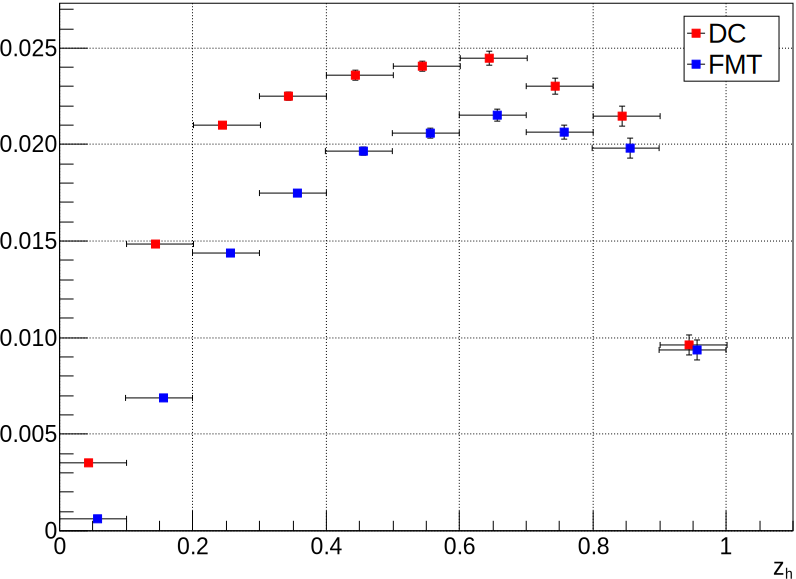
\includegraphics[width=\textwidth]{22zh_acc_-211.pdf}
            \caption{$z_h$ acceptance for $e^-\pi^-$.}
            \label{fig::14.22::zh_acc_-211}
        \end{subfigure}

        \centering
        % pt2 pi+.
        \begin{subfigure}[b]{0.49\textwidth}
            \centering
            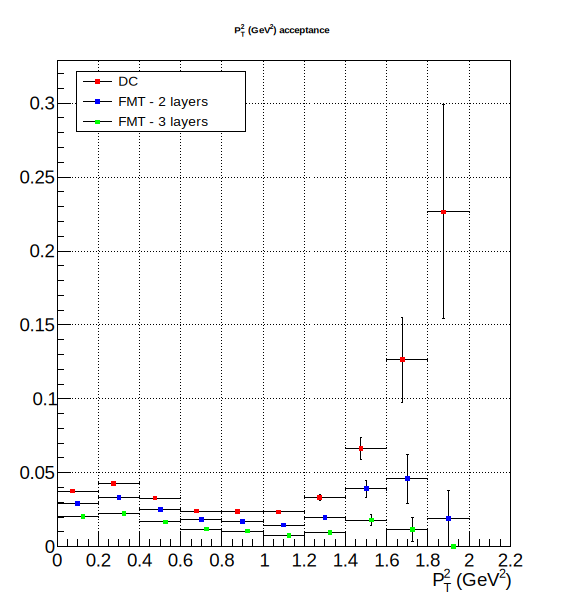
\includegraphics[width=\textwidth]{22pt2_acc_211.pdf}
            \caption{$p_T^2$ acceptance for $e^-\pi^+$.}
            \label{fig::14.22::pt2_acc_211}
        \end{subfigure}
        \hfill
        % pt2 pi-.
        \begin{subfigure}[b]{0.49\textwidth}
            \centering
            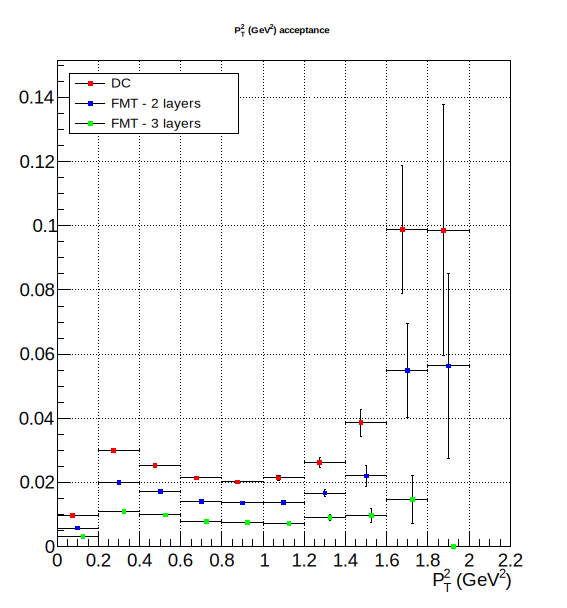
\includegraphics[width=\textwidth]{22pt2_acc_-211.pdf}
            \caption{$p_T^2$ acceptance for $e^-\pi^-$.}
            \label{fig::14.22::pt2_acc_-211}
        \end{subfigure}

        \centering
        % phipq pi+.
        \begin{subfigure}[b]{0.49\textwidth}
            \centering
            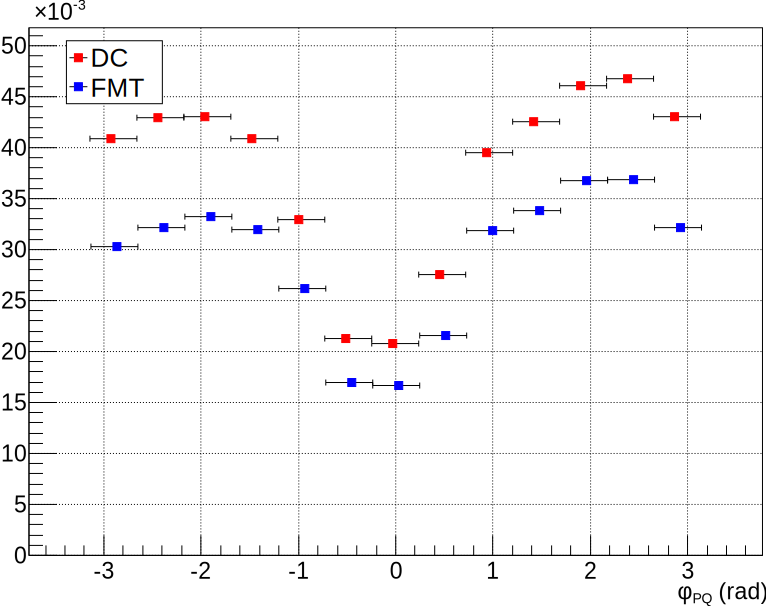
\includegraphics[width=\textwidth]{22phipq_acc_211.pdf}
            \caption{$\phi_{PQ}$ acceptance for $e^-\pi^+$.}
            \label{fig::14.22::phipq_acc_211}
        \end{subfigure}
        \hfill
        % phipq pi-.
        \begin{subfigure}[b]{0.49\textwidth}
            \centering
            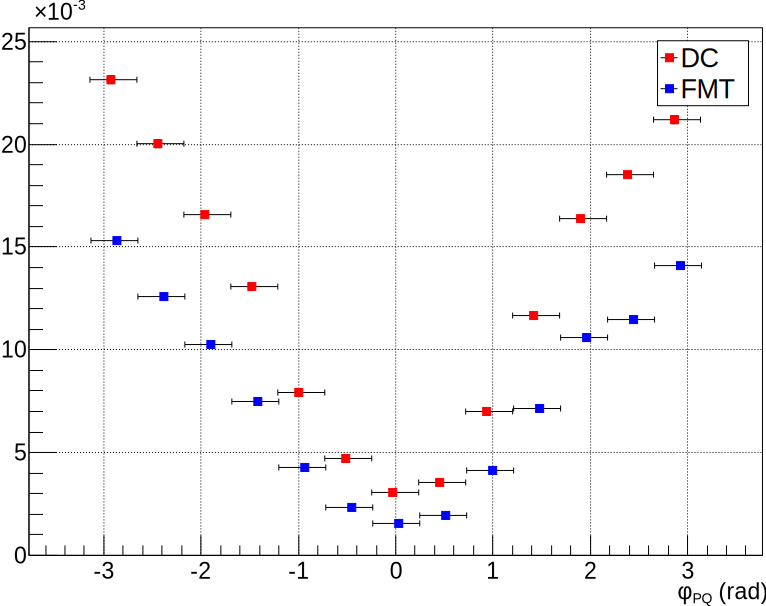
\includegraphics[width=\textwidth]{22phipq_acc_-211.pdf}
            \caption{$\phi_{PQ}$ acceptance for $e^-\pi^-$.}
            \label{fig::14.22::phipq_acc_-211}
        \end{subfigure}
        \caption[hadronic variables acceptance]
        {$z_h$, $p_T^2$, and $\phi_{PQ}$ acceptances for $e^-\pi^+$ and $e^-\pi^-$.
        All electron and other hadronic variables are integrated in all Figures.
        The bin markers are slightly shifted in $x$ to improve legibility.}
        \floatfoot{Source: Own elaboration, using the \href{https://github.com/bleaktwig/clas12-rge-analysis}{clas12-rge-analysis} software.}
        \label{fig::14.22::hadronic_acc}
    \end{figure}


    % !TEX root = ../main.tex
\subsection{Study Results}
\label{14.30::study_results}
    % Explain binning scheme selected.
    To select a region in $v_z$ to place the RG-E target, two criteria were considered: a phase space study and a statistics study.
    In the phase space study, the RG-F target gas region ($-30 < v_z < 20$ cm) was divided into ten 5 cm bins, and the phase space of each kinematic variable was analysed in each bin.
    The results of this study are presented in Section \ref{14.31::phase_space_study}.
    For the statistics study, the region chosen in the phase space study was further divided into 1 cm bins.
    The study aimed to determine which 7 cm region within the chosen range had the largest statistics.
    The validity of this choice was evaluated using a gemc simulation of the RG-E target system.
    The results of this study are presented in Section \ref{14.32::statistics_study}.

    % Statistical error estimation.
    Regarding the statistical error estimation, the total statistical error on the acceptance-corrected result, denoted as $e_\text{corr}$, needs to consider both the statistical error of the measurements ($e_\text{meas}$) and the acceptance correction ($e_\text{acc}$).
    The statistical error of the measurements, $e_\text{meas}$, is purely statistical in nature and is given by
    \begin{equation*}
        e_\text{meas} = \frac{\delta y_\text{meas}}{y_\text{meas}},
    \end{equation*}
    The acceptance correction error, $e_\text{acc}$, was derived in Equation \eqref{eq::14.20::acc_error}.

    Since $e_\text{meas}$ arises purely from experimental data and $e_\text{acc}$ is purely from simulation, they are considered to be completely uncorrelated.
    Therefore, the total statistical error of the acceptance-corrected result can be estimated as the quadratic addition of the two errors, i.e.,
    \begin{equation*}
        e_\text{corr} = \sqrt{e_\text{meas}^2 + e_\text{acc}^2}.
    \end{equation*}

    % !TEX root = ../main.tex
\subsubsection{Phase Space Study}
\label{14.31::phase_space_study}
    % Introduction.
    Considering the objectives of this DIS study, it is advantageous to maximise the phase space of each kinematic variable of study.
    This approach broadens the scope of investigation, increases sensitivity to detect rare phenomena, and facilitates the testing of theoretical predictions for future studies using the double target system.
    Therefore, the first criterion for selecting a $v_z$ region for the target is to find a region that provides the maximum range of kinematic variables.

    % Resulting plots.
    The resulting plots show the acceptance-corrected DIS variables separated into $v_z$ bins.
    Figures \ref{fig::14.31::q2_vz} and \ref{fig::14.31::nu_vz} display the distributions of the electron variables $Q^2$ and $\nu$, respectively.
    The $z_h$ distributions for $e^-\pi^+$ and $e^-\pi^-$ can be observed in Figures \ref{fig::14.31::zh_211_vz} and \ref{fig::14.31::zh_-211_vz}, respectively.
    Figures \ref{fig::14.31::pt2_211_vz} and \ref{fig::14.31::pt2_-211_vz} show the distributions of $p_T^2$ for $e^-\pi^+$ and $e^-\pi^-$, respectively.
    Finally, Figures \ref{fig::14.31::phipq_211_vz} and \ref{fig::14.31::phipq_-211_vz} present the distributions of $\phi_{PQ}$ for $e^-\pi^+$ and $e^-\pi^-$, respectively.
    These plots provide insights into the dependence of each DIS variable on the $v_z$ coordinate.
    For these same distributions without acceptance correction, please see Appendix \ref{20.04::dis_vz_plots}.

    % Q2.
    In the study of $Q^2$, as shown in Figure \ref{fig::14.31::q2_vz}, the higher end of the variable's phase space is limited for $v_z < -5$ cm, with the effect becoming more pronounced as we move further upstream.
    This effect can be understood by considering the compounded effect of the $\theta$ efficiency for negative particles (as seen in Figure \ref{fig::14.21::theta_study_neg}) and the limited acceptance region of FMT (described by Equation \eqref{eq::12.42::fmt_geometry_cut} and illustrated in Figure \ref{eq::12.42::vz_vs_theta}).

    The higher end of $\theta$ becomes limited for lower $v_z$ values.
    Based on the objective of maximising the phase space of each variable, this suggests setting the minimum $v_z$ for the RG-E target near $-5$ cm.
    Additionally, it is noted that the variable exhibits an unusual shape for $10$ cm $< v_z < 20$ cm, likely due to the cut in low $\theta$ angles in that region, which is another consequence of the FMT acceptance region.

    % nu.
    In the study of $\nu$, as seen in Figure \ref{fig::14.31::nu_vz}, it was previously observed that $\nu$ has no direct correlation with the scattering angle $\theta_C$ (Section \ref{14.20::acceptance_correction_results}).
    Therefore, no significant effect on the phase space of $\nu$ is observed for $v_z < -5$ cm, unlike $Q^2$.
    However, a loss is observed in the lower end of the phase space for $v_z = 10$ cm and downstream.
    Based on this effect, it is reasonable to keep $v_z$ below approximately 10 cm to preserve the largest possible phase space of $\nu$.

    % zh.
    In the study of $z_h$, despite its lack of direct correlation with the electron's and pion's $\theta$, clear differences are observed across different $v_z$ bins, as shown in Figures \ref{fig::14.31::zh_211_vz} and \ref{fig::14.31::zh_-211_vz}.
    However, this can be explained by its inverse correlation with $\nu$ (as described in Equation \eqref{eq::10.32::zh}).
    Similar to $\nu$, the extreme phase space loss is primarily observed for $v_z > 10$ cm, and therefore, no additional severe restrictions on the $v_z$ region are imposed beyond those defined based on the studies of $Q^2$ and $\nu$.

    % pt2.
    In the study of $p_T^2$, as depicted in Figures \ref{fig::14.31::pt2_211_vz} and \ref{fig::14.31::pt2_-211_vz}, large statistical fluctuations are observed for $p_T^2 > 1.4 \text{GeV}^2$, consistent with the prediction in Section \ref{14.22::hadronic_variables}.
    Studying the phase space of the variable, a cutoff at high $p_T^2$ values is observed for $v_z < -5$ cm and $v_z > 15$ cm, similar to what was seen for $Q^2$.
    Based on this observation, no additional restrictions are imposed on the $v_z$ region under study.

    % phipq.
    Regarding the study of $\phi_{PQ}$, as shown in Figures \ref{fig::14.31::phipq_211_vz} and \ref{fig::14.31::phipq_-211_vz}, no easily discernible loss is observed in the phase space of $\phi_{PQ}$ as we vary $v_z$.
    While there are significant changes in the shape of the variable distribution across different $v_z$ bins, conducting a detailed shape study is beyond the scope of this thesis, as ample information is already provided by the other DIS variables.

    % !TEX root = ../main.tex
\subsubsection{Statistics Study}
\label{14.32::statistics_study}
    After obtaining the $v_z$ region with the maximum range of kinematic variables, our second criterion is to maximise statistics inside this region.
    With phase space already maximised, this allows us to increase the statistical precision of future studies, enabling a thorough exploration of the parameter space.

    Based on the results of the different phase space studies, we'll limit the scope of this statistics study to the region $-5 \text{cm} < v_z < 10 \text{cm}$, the result of which can be observed in Figure \ref{fig::14.32::statistics}.
    The objective of this study is to find the 7 cm region in $v_z$ with the highest statistics.
    The choice of 7 cm in particular comes from the length of the double target, where the liquid target has a length of 3 cm, the separation between the liquid and solid target is 4 cm, and the solid target is of negligible width for the scope of this study.

    First, we look at $e^-$ statistics, seen in Figure \ref{fig::14.32::statistics_11}.
    It is trivial to note that, in the studied range, the more upstream we look, the more statistics are seen.
    Therefore, the best region for the placement of the target is from $-5$ to $2$ cm.
    This result is only reinforced by the results observed in $e^-\pi^+$ and $e^-\pi^-$ statistics, which can be seen in Figures \ref{fig::14.32::statistics_211} and \ref{fig::14.32::statistics_-211}.

    % statistics.
    \begin{figure}
        \centering
        % e-.
        \begin{subfigure}[b]{\textwidth}
            \centering
            \includegraphics[width=\textwidth]{32statistics_11.png}
            \caption{$e^-$ statistics.}
            \label{fig::14.32::statistics_11}
        \end{subfigure}
        \centering
        % e-pi+.
        \begin{subfigure}[b]{0.49\textwidth}
            \centering
            \includegraphics[width=\textwidth]{32statistics_211.png}
            \caption{$e^-\pi^+$ statistics.}
            \label{fig::14.32::statistics_211}
        \end{subfigure}
        \hfill
        % e-pi-.
        \begin{subfigure}[b]{0.49\textwidth}
            \centering
            \includegraphics[width=\textwidth]{32statistics_-211.png}
            \caption{$e^-\pi^-$ statistics.}
            \label{fig::14.32::statistics_-211}
        \end{subfigure}
        \caption[Statistics for $e^-$, $e^-\pi^+$, and $e^-\pi^-$ against $v_z$]
        {$e^-$, $e^-\pi^+$, and $e^-\pi^-$ statistics against $v_z$ for run 12016.
        No acceptance correction was applied to these results.}
        \floatfoot{Source: Own elaboration, using the \href{https://github.com/bleaktwig/clas12-rge-analysis}{clas12-rge-analysis} software.}
        \label{fig::14.32::statistics}
    \end{figure}


    % Q2.
    \begin{figure}
        \centering
        \includegraphics[width=\textwidth]{31q2_vz.png}
        \caption[Acceptance-corrected $Q^2$ separated in $v_z$ bins]
        {Acceptance-corrected $Q^2$ detected by DC and FMT, separated in $v_z$ bins.
        Run 12016.
        The bin markers are slightly shifted in $x$ to improve legibility.}
        \floatfoot{Source: Own elaboration, using the \href{https://github.com/bleaktwig/clas12-rge-analysis}{clas12-rge-analysis} software.}
        \label{fig::14.31::q2_vz}
    \end{figure}

    % nu.
    \begin{figure}
        \centering
        \includegraphics[width=\textwidth]{31nu_vz.png}
        \caption[Acceptance-corrected $\nu$ separated in $v_z$ bins]
        {Acceptance-corrected $\nu$ detected by DC and FMT, separated in $v_z$ bins.
        Run 12016.
        The bin markers are slightly shifted in $x$ to improve legibility.}
        \floatfoot{Source: Own elaboration, using the \href{https://github.com/bleaktwig/clas12-rge-analysis}{clas12-rge-analysis} software.}
        \label{fig::14.31::nu_vz}
    \end{figure}

    % zh.
    \begin{figure}
        \centering
        \includegraphics[width=\textwidth]{31zh_vz_211.png}
        \caption[Acceptance-corrected $z_h$ for $e^-\pi^+$ separated in $v_z$ bins]
        {Acceptance-corrected $z_h$ for $e^-\pi^+$ detected by DC and FMT, separated in $v_z$ bins.
        Run 12016.
        The bin markers are slightly shifted in $x$ to improve legibility.}
        \floatfoot{Source: Own elaboration, using the \href{https://github.com/bleaktwig/clas12-rge-analysis}{clas12-rge-analysis} software.}
        \label{fig::14.31::zh_211_vz}
    \end{figure}

    \begin{figure}
        \centering
        \includegraphics[width=\textwidth]{31zh_vz_-211.png}
        \caption[Acceptance-corrected $z_h$ for $e^-\pi^-$ separated in $v_z$ bins]
        {Acceptance-corrected $z_h$ for $e^-\pi^-$ detected by DC and FMT, separated in $v_z$ bins.
        Run 12016.
        The bin markers are slightly shifted in $x$ to improve legibility.}
        \floatfoot{Source: Own elaboration, using the \href{https://github.com/bleaktwig/clas12-rge-analysis}{clas12-rge-analysis} software.}
        \label{fig::14.31::zh_-211_vz}
    \end{figure}

    % pt2.
    \begin{figure}
        \centering
        \includegraphics[width=\textwidth]{31pt2_vz_211.png}
        \caption[Acceptance-corrected $p_T^2$ for $e^-\pi^+$ separated in $v_z$ bins]
        {Acceptance-corrected $p_T^2$ for $e^-\pi^+$ detected by DC and FMT, separated in $v_z$ bins.
        Run 12016.
        The bin markers are slightly shifted in $x$ to improve legibility.}
        \floatfoot{Source: Own elaboration, using the \href{https://github.com/bleaktwig/clas12-rge-analysis}{clas12-rge-analysis} software.}
        \label{fig::14.31::pt2_211_vz}
    \end{figure}

    \begin{figure}
        \centering
        \includegraphics[width=\textwidth]{31pt2_vz_-211.png}
        \caption[Acceptance-corrected $p_T^2$ for $e^-\pi^-$ separated in $v_z$ bins]
        {Acceptance-corrected $p_T^2$ for $e^-\pi^-$ detected by DC and FMT, separated in $v_z$ bins.
        Run 12016.
        The bin markers are slightly shifted in $x$ to improve legibility.}
        \floatfoot{Source: Own elaboration, using the \href{https://github.com/bleaktwig/clas12-rge-analysis}{clas12-rge-analysis} software.}
        \label{fig::14.31::pt2_-211_vz}
    \end{figure}

    % phipq.
    \begin{figure}
        \centering
        \includegraphics[width=\textwidth]{31phipq_vz_211.png}
        \caption[Acceptance-corrected $\phi_{PQ}$ for $e^-\pi^+$ separated in $v_z$ bins]
        {Acceptance-corrected $\phi_{PQ}$ for $e^-\pi^+$ detected by DC and FMT, separated in $v_z$ bins.
        Run 12016.
        The bin markers are slightly shifted in $x$ to improve legibility.}
        \floatfoot{Source: Own elaboration, using the \href{https://github.com/bleaktwig/clas12-rge-analysis}{clas12-rge-analysis} software.}
        \label{fig::14.31::phipq_211_vz}
    \end{figure}

    \begin{figure}
        \centering
        \includegraphics[width=\textwidth]{31phipq_vz_-211.png}
        \caption[Acceptance-corrected $\phi_{PQ}$ for $e^-\pi^-$ separated in $v_z$ bins]
        {Acceptance-corrected $\phi_{PQ}$ for $e^-\pi^-$ detected by DC and FMT, separated in $v_z$ bins.
        Run 12016.
        The bin markers are slightly shifted in $x$ to improve legibility.}
        \floatfoot{Source: Own elaboration, using the \href{https://github.com/bleaktwig/clas12-rge-analysis}{clas12-rge-analysis} software.}
        \label{fig::14.31::phipq_-211_vz}
    \end{figure}

    % statistics.
    \begin{figure}
        \centering
        % e-.
        \begin{subfigure}[b]{\textwidth}
            \centering
            \includegraphics[width=\textwidth]{32statistics_11.png}
            \caption{$e^-$ statistics.}
            \label{fig::14.32::statistics_11}
        \end{subfigure}
        \centering
        % e-pi+.
        \begin{subfigure}[b]{0.49\textwidth}
            \centering
            \includegraphics[width=\textwidth]{32statistics_211.png}
            \caption{$e^-\pi^+$ statistics.}
            \label{fig::14.32::statistics_211}
        \end{subfigure}
        \hfill
        % e-pi-.
        \begin{subfigure}[b]{0.49\textwidth}
            \centering
            \includegraphics[width=\textwidth]{32statistics_-211.png}
            \caption{$e^-\pi^-$ statistics.}
            \label{fig::14.32::statistics_-211}
        \end{subfigure}
        \caption[Statistics for $e^-$, $e^-\pi^+$, and $e^-\pi^-$ against $v_z$]
        {$e^-$, $e^-\pi^+$, and $e^-\pi^-$ statistics against $v_z$ for run 12016.
        No acceptance correction was applied to these results.}
        \floatfoot{Source: Own elaboration, using the \href{https://github.com/bleaktwig/clas12-rge-analysis}{clas12-rge-analysis} software.}
        \label{fig::14.32::statistics}
    \end{figure}


% \subsection{Conclusions}
% TODO. Something something something.
% TODO. Mention issue of large systematic errors (~10%) not considered in the work.
%   * TODO. Ask Raffaella for a reference about the "average" systematic error I should consider.
